\chapter{A brief introduction to electric charges, currents, fields and potentials}
\label{chap:Basics}
%%% fref fixed

Neural activity is generated by electric currents that go through neural membranes. In turn, these currents
evoke the extracellular electric potentials that are the main topic of this book.

Before we talk more about the electric signaling in the brain, we will in this chapter give a general introduction to electromagnetic theory, focusing mostly on the electric part of it, and less on the magnetic. The aim of this rather incomplete introduction is to establish an elementary understanding of the main concepts that we will use in the remainder of this book.

Electromagnetic theory is summarized by Maxwell's equations, and we might have kick-started this chapter by listing up those. However, since Maxwell's equations may appear a bit challenging for "the untrained eye", we will be taking a "softer" path, which we deem sufficient for establishing the main concepts that we will be working with. For good taste and later reference, we nevertheless go through Maxwell's equations in the final part of the chapter (Section \ref{sec:Basics:Maxwell}). Towards the end of the chapter we will also go through some of the most important assumptions that we use when applying the electromagnetic theory to predict electric potentials in complex medium like brain tissue.

Readers without prior schooling in physics might not be able to follow all parts of this introduction, but it will hopefully still give them a basic understanding of the concepts of \textit{electric charge}, \textit{electric currents}, \textit{electric fields}, and \textit{electric potentials}, and some insight into how they are related to one another. Readers that do have a physics background might see the first part of this introduction as a useful repetition, and may appreciate the later parts, which deal with less trivial issues regarding the use of electromagnetic theory in a complex medium such as brain tissue.



\section{\blue{Electric charge}}
\label{sec:Basics:Charge} \index{Charge}
Let us begin with the fundamental quantity for electricity, the electric charge. Nature's fundamental charges are those carried by the protons and electrons that build up the atoms that build up the material world. The proton carries the charge $e$, while the electron carries the charge $-e$, where $e = 1.602\times10^{-19}$ coulomb (\si{\coulomb}) is called the \textit{unit charge} \index{Unit charge}.

Since atoms in their natural state contain an equal number of electrons and protons, most matter is electrically neutral. Some mediums are nevertheless conductive, which means that they contain so-called "free charge carriers" that may move through the medium. In an electric copper cable, such as that carrying current to normal desktop lamp, the free charge carriers are electrons that are not bound to specific locations (i.e., to specific copper atoms), but can move freely through the copper material. In an electrolyte solution, for example salt-water (saline), the free charge carriers are instead ions, i.e., atoms or molecules that have gained or donated one or several electrons, and therefore have become electrically charged. The saline solutions that fill the intracellular and extracellular space of the brain are such electrolytic solutions. Important charge carriers in the brain are sodium and potassium ions (Na$^+$ and K$^+$ with charge $1e$), chloride ions (Cl$^-$ with charge $-1e$), and calcium ions (Ca$^{2+}$ with charge $2e$).

At a fundamental, microscopic level, electricity is due to the movement of charges. Such a movement can be caused both by electric and magnetic forces, but for now, we consider only the electric force, which is the most important for the phenomena that we will study in this book. A pair of charges, $q_1$ and $q_2$, will act on each others with a force $F$ (with units newton (\si{\newton})) given by Coulomb's law:
\begin{equation}
F = \frac{q_1q_2}{4\pi \epsilon_0} \frac{1}{r^2},
\label{eq:Basics:CoulombF}
\end{equation}
where the constant $\epsilon_0$ is the permittivity of free space, and $r$ is the distance between the two charges. The direction of the force is along the line between the two charges, and the force is inversely proportional to the square of the distance between them. The force will be repelling if the charges have the same sign and attractive if they have the opposite sign. 

We can express the direction of the force mathematically by use of a vector notation. Letting a boldface notation indicate that an entity is a vector, we denote the positions of the charges $q_1$ and $q_2$ by ${\bf r}_1$ and ${\bf r}_2$, respectively. The position vector ${\bf r}_1$ can be visualized as an arrow from some reference point ${\bf r} =0$ to the position of the charge $q_1$. Likewise, the vector ${\bf r}_1-{\bf r}_2$ can be visualized as an arrow from the position of $q_2$ to the position of $q_1$, defining both the distance and direction of the (imagined) line connecting them. In vector notation, the force between the charge pair can be written:
\begin{equation}
{\bf F} = \frac{q_1q_2}{4\pi \epsilon_0 |{\bf r}_1-{\bf r}_2|^2} \hat{{\bf r}}_{1,2}.
\label{eq:Basics:CoulombFvec}
\end{equation}
We have here introduced the \textit{unit vector},
\begin{equation}
\hat{{\bf r}}_{1,2} = \frac{{\bf r}_1 - {\bf r}_2}{|{\bf r}_1-{\bf r}_2|},
\label{eq:Basics:UnitVector}
\end{equation}
defined as vector ${\bf r}_1-{\bf r}_2$ divided by its own length $|{\bf r}_1-{\bf r}_2|$, so that its length is one (unity). We chose this notation because the unit vector defines the direction of the force, but says nothing about its magnitude, while the fraction in front of it is a scalar (a number with no direction) that defines the magnitude of the force, but  says nothing about its direction. It is then easy to verify that the magnitude is the same as in \fref{eq:Basics:CoulombF}.

If there are several ($N$) point charges present, the contribution from each of them sum up linearly. If we have a charge $q_1$ in a position ${\bf r}_1$, the force acting on it by the $N-1$ other charges $q_2, q_3, q_4 ... q_{N}$ in positions ${\bf r}_2, {\bf r}_3, {\bf r}_4 ... {\bf r}_{N}$ will be:
\begin{equation}
{\bf F}({\bf r_1}) = \sum_{n=2}^{N} \frac{q_1 q_n}{4\pi \epsilon_0} \frac{\hat{{\bf r}}_{1,n}}{|{\bf r}_1-{\bf r}_n|^2}.
\label{eq:Basics:CoulombFN}
\end{equation}

If our system of study consisted of a small number $N$ of charges, we could use $N$ instances of \fref{eq:Basics:CoulombFN} to compute the force acting on all the $N$ individual charges. Together with Newton's law ${\bf F} = m {\bf a}$, which tells us how the charges will be accelerated in the force direction, \fref{eq:Basics:CoulombFN} would then allow us to compute the movements of all our charges over time.

Although \fref{eq:Basics:CoulombFN} establishes the fundamental origin for electric interactions, there is a fairly long way to go from this equation to the understanding of electric phenomena in a macroscopic system such as for example the brain. When describing a macroscopic system, we are usually not interested in the microscopic interactions between a small number of charges, but rather the joint interactions of a very, very large number of charges. It is then not feasible to keep record of the position of each individual charge, but rather to work with continuous variables defined on a larger spatial scale, such as charge densities, $\rho$ (with units \si{\coulomb\per\cubic\metre}), or ion concentrations, $c_k$ (with units millimolar ($1\, \si{\milli\molar} = 1 \,\si{\mole\per\cubic\metre} = 6.02\times10^{23}$ particles per \si{\cubic\metre}). The movement of particles of a given species $k$ is then quantified in terms of a particle flux, $J_k$, with units \si{\mole\per\second}, and the movement of charge is quantified in terms of an electric current, $I$, with units Ampere (\si{\ampere} = \si{\coulomb\per\second}).

\gen{I tillegg kan det jo ogsaa vaere magnetiske krefter paa ladninger, kanskje bare nevne det for "completeness"?}
\ghnote{La til kort kommentar i begynnelsen.}


\section{\blue{Electric fields and potentials}}
\label{sec:Basics:Fields} \index{Electric field}
The electric field at a given location (with units volts per metre (\si{\volt\per\metre})) can be defined as the electric force that would act on a reference charge $q$ if it were present there, i.e.,
\begin{equation}
{\bf E}({\bf r}) = {\bf F}({\bf r})/q.
\label{eq:Basics:E}
\end{equation}
Since the electric force is due to the Coulomb force, the electric field generated by $N$ charges can be obtained by inserting \fref{eq:Basics:CoulombFN} into \fref{eq:Basics:E}:
\begin{equation}
{\bf E}({\bf r}) = \sum_{n=1}^{N}  \frac{q_n}{4\pi \epsilon_0} \frac{\hat{{\bf r}}_{1,n}}{|{\bf r}-{\bf r}_n|^2}.
\label{eq:Basics:CoulombEN}
\end{equation}

Tightly related to the electric field ${\bf E}$ is the electric potential $\phi$ (with units volts (\si{\volt})), which is what we normally measure experimentally with electrodes \index{Electric potential}. While ${\bf E}$ is a fundamental physical entity, $\phi$ may be regarded as an auxiliary variable. It is a way to represent the electric field that often makes computations simpler and measurements easier.

The electric field can be expressed as the spatial derivative, or gradient, of the potential:
\begin{equation}
{\bf E}(x,y,z) = - {\bf \nabla} \phi(x,y,z) = - \left(\frac{d\phi}{dx} {\bf e}_x  + \frac{d\phi}{dy} {\bf e}_y + \frac{d\phi}{dz} {\bf e}_z \right) \phi.
\label{eq:Basics:EV}
\end{equation}
The operator ${\bf \nabla}$ computes a property's spatial rate of change (also called the gradient) in the various spatial directions, and ${\bf e}_x$, ${\bf e}_y$ and  ${\bf e}_z$ are the unit vectors in the three spatial directions $x$, $y$ and $z$, respectively.

For a spherical symmetric potential,
\begin{equation}
{\bf \nabla} \phi(r) = \frac{d\phi(r)}{dr} {\bf \hat{r}}.
\label{eq:Basics:SphericalNablaPhi}
\end{equation}
Since the field contribution from each point charge is spherically symmetric around its position (${\bf r}_n$), the field in \fref{eq:Basics:CoulombEN} can thus be written as the gradient of the potential:
\begin{equation}
{\phi}({\bf r}) = \sum_{n=1}^{N}  \frac{q_n}{4\pi \epsilon_0} \frac{\hat{{\bf r}}_{1,n}}{|{\bf r}-{\bf r_n}|}.
\label{eq:Basics:CoulombPhiN}
\end{equation}

Unlike ${\bf E}$, which is a vector field, $\phi$ is a scalar field, and as such, tends to be easier to deal with because measuring the value of a vector field requires measurement in all three spatial dimensions. We note that \fref{eq:Basics:EV} rests on something called the \textit{quasi-static approximation} of Maxwell's equations, which we explain further in \fref{sec:Basics:Maxwell}.

\gen{Senere har vi vel brukt andre symboler for potensial, i alle fall jeg.} \ghnote{Vi maa bestemme oss der, ja. Jeg og Torbjorn har brukt $\phi$, Gaute har brukt $V$, men jeg har brukt $V$ for membranpotensialet. }\gen{I Sterratt bruker vi $V_e/V_i$ for ekstracellulaert/intracellulaert potentsial, og $V$ for membranpotensial. Generelt fint hvis vi kan bruke mest mulig samme notasjon her, synes jeg}


\subsection{\blue{Electric ground}}
\label{sec:Basics:Ground}
To get an intuitive understanding of the relationship between ${\bf E}$ and $\phi$, it helps to consider an idealized one-dimensional scenario with a constant field in the $x$-direction. Then, \fref{eq:Basics:EV} simplifies to,
\begin{equation}
E = -\frac{d\phi(x)}{dx} = -\frac{\Delta \phi}{\Delta x} = -\frac{\phi(x_b)-\phi(x_a)}{x_b-x_a},
\label{eq:Basics:EV1D}
\end{equation}
where the first equality follows from the 1D-assumption, the second from the assumption that $E$ is constant, and the third is simply a definition of the second, where $x_b$ and $x_a$ may represent any two arbitrary points in space. For example, if $E = 1$~\si{\volt\per\metre}, and the distance between our points $x_b-x_a$ is 1~\si{\metre}, \fref{eq:Basics:EV1D} tells us that $\phi$ will be 1~\si{\volt} lower in $x_b$ compared to $x_a$ (\fref{fig:Basics:Ground}).

\begin{figure}[!ht]
\begin{center}
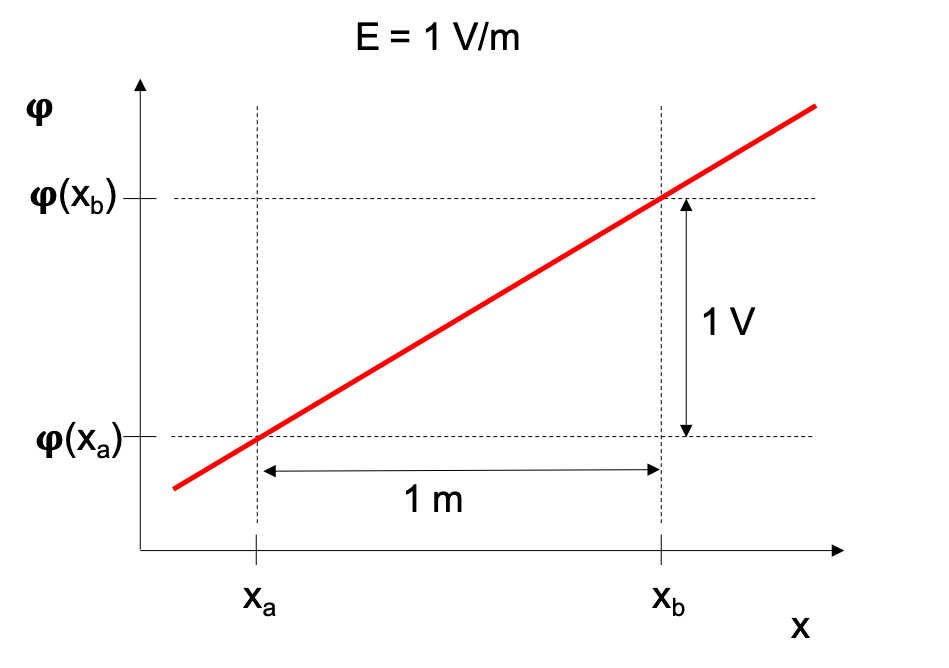
\includegraphics[width=0.8\textwidth]{Figures/Basics/Ground.png}
\end{center}
\caption{\textbf{Relationship between the electric field and electric potential.} With a constant electric field $E = 1\,\si{\volt\per\metre}$, the electric potential $\phi$ increases linearly with distance $x$. With two locations $x_a$ and $x_b$ 1~\si{\metre} apart, we know that $\phi(x_b) = \phi(x_a) + 1\,\si{\volt}$. We are free to define an arbitrary reference point (ground) for the $\phi$, and if we take $\phi(x_a) = 0$, it follows that $\phi(x) = (x-x_a)E$. In $x_b$, we then get $\phi(x_b)=(1\,\si{\metre})\times(1\, \si{\volt\per\metre}) =1\,\si{\volt}$. Equivalently, we might define $x_b$ as our reference point, which would mean that $\phi(x_b) = 0$ and $\phi(x_a) = -1\,\si{\volt}$. Regardless of where we place our reference point, the physics (i.e., the field, $E$) would be the same.
}
\label{fig:Basics:Ground}
\end{figure}

We may use the example in \fref{fig:Basics:Ground} to define the important concept of \textit{ground}\index{Ground}. The field ${\bf E}$ generally determines the potential only up to a constant. In the example, the field $E = 1$ V/m would be consistent with any pair of potentials $\phi_a$ and $\phi_b$ as long as $\phi_b - \phi_a =  1 \,\si{\volt}$. Since it is the field, and not the potential, that is the fundamental physical entity, we can therefore not speak of the potential in a certain point as an absolute entity, but only the potential \textit{difference} between two points. When we measure the potential in a given location, it is always measured relative to some reference electrode (\fref{fig:Basics:elec_circuit}), which we often call \textit{ground}, and where we define $\phi = 0$ (cf. example in \Fref{fig:Basics:Ground}). When we record extracellular potentials in the brain, we can choose to place the reference electrode close or far away from the recording electrode, depending on the kind of signal one wishes to measure \cite**{Sharott2015}. 

By definition, the electric potential is the energy needed to move a unit of electric charge $q$ from the reference point (ground) to a specific location in the electric field (\fref{fig:Basics:elec_circuit}). The unit (V) of the electric potential is equivalent to energy per charge, or Joule per Coulomb (1 \si{\volt} = 1 \si{\joule\per\coulomb}). As such, the concept of an electric potential is closely related to the concept of a potential energy. The potential energy ($U_E$) of a charge $q$ in an electric field is:
\begin{equation}
U_E = q\phi.
\label{eq:Basics:UE}
\end{equation}
\tvnnote{Link this to neuroscience measurements and currents.}
\ghnote{Hva mener du?}

\begin{figure}[!ht]
\begin{center}
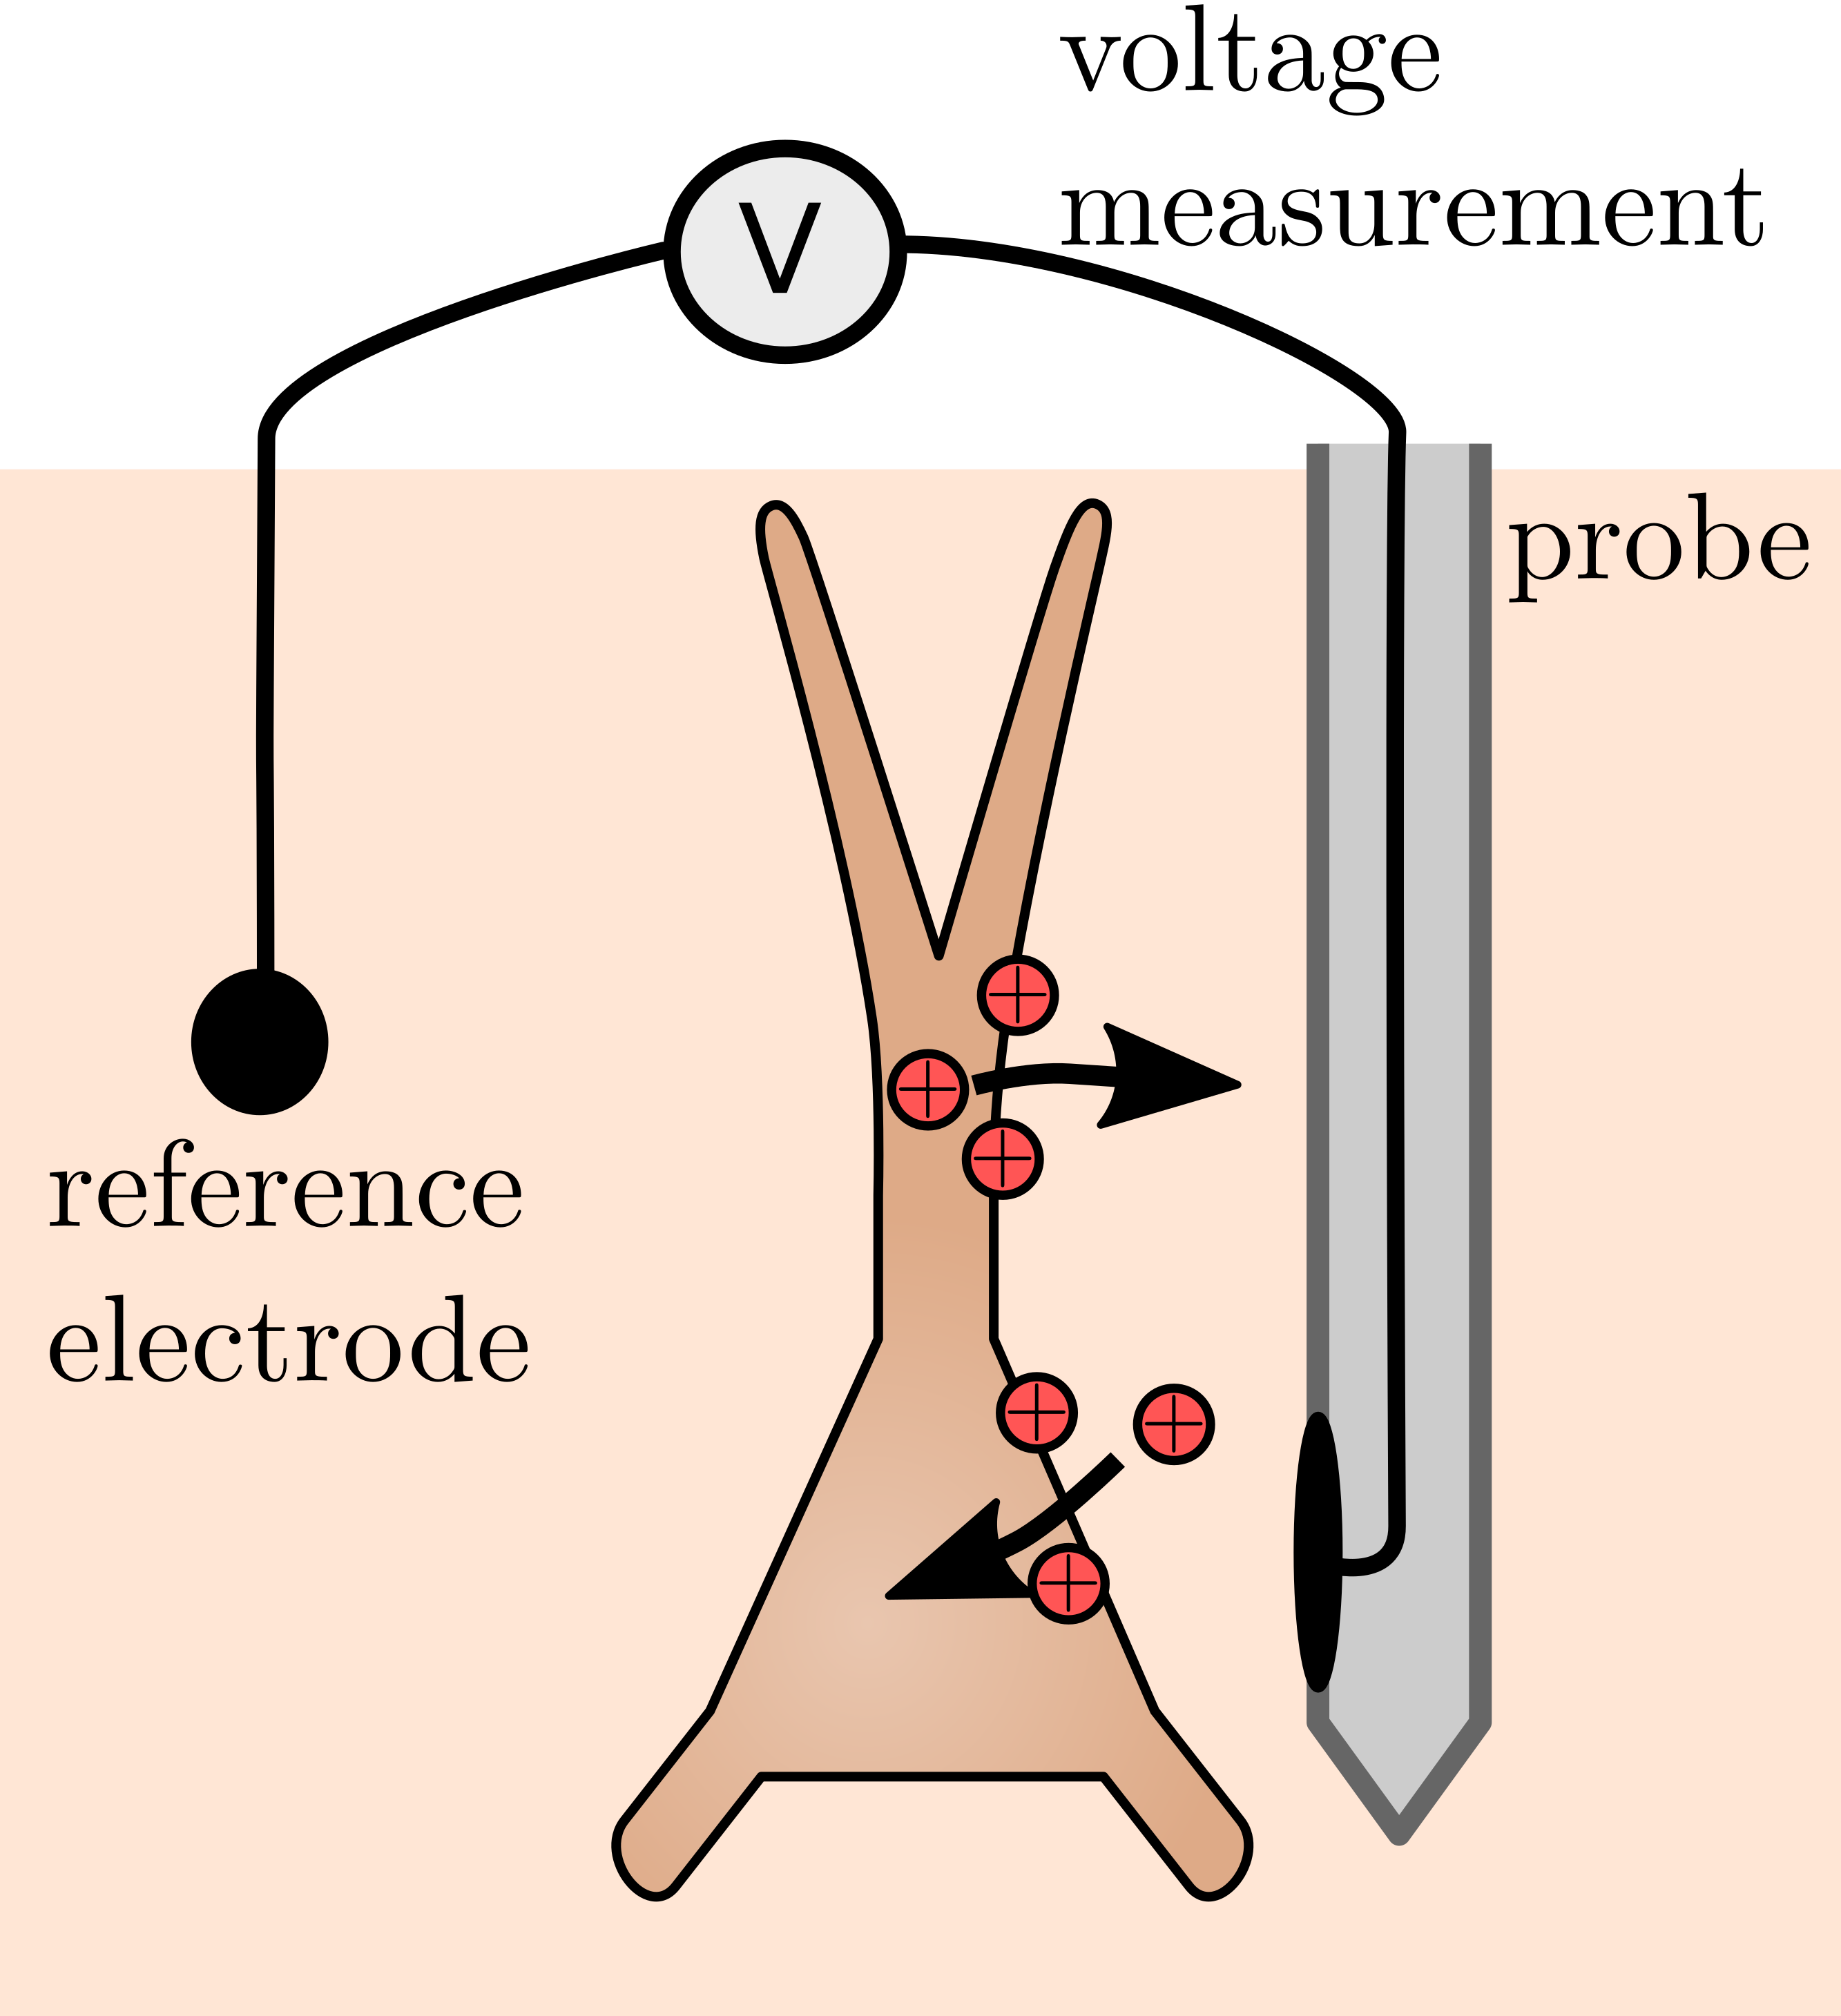
\includegraphics[width=0.4\textwidth]{Figures/Basics/rec_elec_circuit.png}
\end{center}
\caption[]{\textbf{Measurement of extracellular potential.}
Electric potential is measured between recording electrode and reference electrode, and represents the energy required to move a positive test charge from the reference electrode to the measurement electrode. If, say, positive ions are leaving the extracellular medium (and entering a cell) in the vicinity of the recording electrode, then the energy needed to move a positive charge to the measurement electrode is negative, that is, one can gain energy by moving the charge there.}
\label{fig:Basics:elec_circuit}
\end{figure}

\ghnote{Mulig vi burde diskutere plassering av referanseelektrode grundigere, men jeg holdt det paa et minumum her.}
\gen{Kanskje si enda klarere at man oensker at potensialet paa referanseelektroden skal vaere saa konstant som mulig under eksperimentet (eller blir dette sirkulaert?), husker at Anna plasserte referanseelektroden i nakken paa rottene hun gjorde maalinger fra. Kanskje vi kan hoere med eksperimentalistene paa CINPLA hva de gjoer?} \ghnote{Sikkert lurt aa spoerre noen, ja, men saa vidt jeg skjoenner er dette et vanskelig spoersmaal der mange avveininger maa gjoeres. Foreslaar at vi flytter dette stoffet et annet sted.}
 

\subsection{\blue{Electroneutrality and Debye shielding}}
\label{sec:Basics:Debye}
Above, we saw that the electric potential resulting from a certain known arrangement of charges is given by \fref{eq:Basics:CoulombPhiN}. This formula works very well for textbook physics examples considering a few bound charges in a non-conducting material or in vacuum, but it is not very useful for studying processes taking place on a larger spatial scale in a conducting material. The reason is that a conducting material is densely packed with free charges that are constantly interacting and in constant motion. 

The Coulomb force (\fref{eq:Basics:CoulombF}) will make each of these charges attract charges of opposite sign and repel charges of the same sign. An individual positive charge in a conductive medium will therefore be immediately surrounded by negative charges, and vice versa, which very effectively shields the potential from the charge. This phenomenon is known as Debye screening or Debye shielding\index{Debye shielding}. 

We know from \textit{Debye-H{\"u}ckel theory}, which we do not present in any detail here, that the shielding effects in a conduction medium will cause the potential to decay \textit{not} as:
\begin{equation}
\phi(r) = \frac{q}{4\pi \epsilon_0 r}, 
\label{eq:Basics:Coulomb_phi1}
\end{equation}
which is the single charge version of \fref{eq:Basics:CoulombPhiN}, but instead as:
\begin{equation}
\phi(r) = \frac{q}{4\pi \epsilon_0 \epsilon_r r} e^{-r/r_D}.
\label{eq:Basics:DebyeScreening}
\end{equation}
Here, $r_D$ is called the \textit{Debye shielding distance} and $\epsilon_r$ is the \textit{relative permittivity} of the medium, which has a value of about 80 in water and dilute saline solutions \cite**{hasted1948}. In the saline solution in the brain, $r_D$ is typically just below 1 \si{\nano\metre} \cite**{Hille2001}, which implies that any given reference charge will give a negligible contribution to the potential at distances larger than the nanometre scale.

Closely related to the discussion above is the concept of electroneutrality\index{Electroneutrality}. When arranged by Coulomb interactions, the numbers of positive and negative charges within a finite and not too small volume of space tend to be kept in close balance. If this were not the case, and a reference volume of tissue did contain a net charge density $\rho$, the very strong Coulomb forces associated with it would cause $\rho$ to decay to zero at a rate proportional to the so-called \textit{charge-relaxation time}, which in brain tissue is on the order of a nanosecond (see \fref{sec:Basics:Quasimagnetostatic}). On spatial scales larger than nanometres and temporal scales larger than nanoseconds, brain tissue will therefore to a good approximation be practically electroneutral \cite**{Nunez2006,Grodzinsky2011}.

Since charges are free to move around both inside and outside cells, both the intracellular domain and the extracellular domain are practically electroneutral. However, whereas the intra- and extracellular mediums are conducting, the cellular membrane is largely dielectric (inslulating), and violations of electroneutrality can therefore occur locally at neural membranes.
Due to the capacitive properties of neural membranes (see \fref{sec:Basics:CapacitiveCurrent}), a patch of membrane can separate a charge $-q$ on the interior side from a charge $q$ on the exterior side, and this breach of electroneutrality is what gives rise to the membrane potential. However, since the membrane is just some nanometres thick, the separation of $-q$ from $q$ occurs on a small spatial scale, and the two charges will still shield each others' contributions to the electric potential some nanometres away from the membrane. 

The practical implication of electroneutrality and shielding effects is that, when we study extracellular potentials (or fields), we can neglect contributions from any particular distribution of charges, and instead compute extracellular potentials from the constraint or current continuity, or equivalently, the constraint that  there should be no charge accumulation anywhere in the extracellular space. As we shall see, it will then be the current sources at neural membranes that give rise to an extracellular potential $\phi$. For example, consider positive ions flowing through the neural membrane into a cell, thereby leaving a certain region of the extracellular medium. This will cause a rearrangement of the extracellular ions, so that positive ions move into this region and negative ions move out from this region. The potential can then be thought of, not as a the result of a particular charge-distribution, but rather as a higher level entity, reflecting the energy landscape needed for these ionic movements to take place in a manner that preserves electroneutrality. 

As we noted earlier, the charge-relaxation time in the extracellular saline solution is on the order of a nanosecond. In comparison, the timescale of neural transmembrane currents tends to be milliseconds (\fref{chap:Neuron}). The gives the charge-relaxation processes a good margin for keeping up with the neural activity. For practical purposes, we can therefore assume that the relationship between transmembrane neural currents and the extracellular potential is instantaneous.


\ghnote{Flyttet samtlige kommentarer til delkapittelet hit, og svarer paa dem her:} \tvnnote{Might be a good place to go through the key points in Exercise 1 in our course, to illustrate how small this breach of electroneutrality really is?}. \ghnote{Ex 1 shows that the number of unbalanced unit charges inside a compartment (e.g., soma) is small compared to the total number of ions in the compartment. However, the unbalanced charges are stuck on the membrane, while the "rest" of the compartment is electroneutral. I do not think it is easy to relate that to the point that we needed to make in this passage of the book. Here, the point is that the unbalanced membrane charges on the in- and outside are close in space, and therefore shield each-other on the spatial scale relevant for us.} \gen{Kanskje si eksplisitt at mens intracellular og ekstracellular "medium" kan sees paa som en "conductor", saa kan selve membranen sees paa som et isolerende dielektrikum (hvis en tenker paa vanlig elektrisk klassifisering av materialer)?} \ghnote{La inn kort kommentar i setningen over.} \gen{Si noe om at dette tilsvarer aa jobbe med ionekonsentrasjoner, istedenfor enkeltioner (hvis dette er riktig)?} \ghnote{Ja, puttet det inn lenger oppe, i seksjonen om "charges".}

\gen{Kanskje spesielt nevne noe om at folk med bakgrunn i fysikk ofte tenker paa hjernen som et dielektrikum (som ofte er tema i vanlige fysikkurs) og ikke som en conductor. En grunn til dette kan vaere at den matematiske formelen for potensialet rundt en stromkilde i en leder, er den samme som for potensialet rundt en ladning i et dielektrikum.}




% On a microscopic scale, we would expect a reference charge to evoke a potential given by the single charge version of \fref{eq:Basics:CoulombPhiN}, i.e., by:
%\begin{equation}
%\phi(r) = \frac{q}{4\pi \epsilon_0 r}.
%\label{eq:Basics:Coulomb_phi1}
%\end{equation}
%However, according to
%As the Coulomb force (\fref{eq:Basics:CoulombFN}) applies to a microscopic scale, so will the resulting electric field (\fref{eq:Basics:CoulombEN}) and potential (\fref{eq:Basics:CoulombPhiN}). The potential ${\phi}({\bf r})$ predicted from \fref{eq:Basics:CoulombPhiN} will therefore depend strongly on the distance to the nearest charge ($|{\bf r}-{\bf r_n}|$). Macroscopic media are normally densely packed with charges. For example, in the saline solution of the brain the average intra-charge distance is on the order of a nanometre\tvnnote{cite?}, which means that the potential will vary strongly with a sub-nanometre resolution\tvnnote{Isn't this only true if we assume that the charges are held in place? Presumably it wouldn't actually take substantially more energy to move a charge here, because it would only push away a charge by a few nanometres?}. A direct use of \fref{eq:Basics:CoulombPhiN} will therefore, again, force us to keep track of each individual charge, which would not be feasible in a macroscopic system.
%Fortunately, we do not need to care too much about these microscopic field variations when we are trying to understand the brain.
%\gen{Boer kanskje si noe om hvilke spoersmaal man da begrenser seg til? Er neglisjering av microscopic field variations det samme som aa anta
%kontinuumapproksimasjon for elektrisk stroemmer? Og den kan generelt ikke brukes for detaljert modellering av stroem gjennom ionekanaler basert paa molekylaerdynamikk, slik jeg har forst{\aa}tt det.} A technical argument for why, is that the electrodes used to record brain signals have a tip diameter which is typically a micrometre or more. This is much larger than the average intra-charge distance in the saline solution of the brain. The electrodes therefore do not "sense" the microscopic fluctuations, but rather the average field taken over the electrode surface.
%\gen{"Surface" faar meg til kun aa tenke paa metallelektroder. Kanskje legge et ord eller to slik at liquid-elektroder ogsaa er dekket?}
%When we speak of an electric field or electric potential in the brain, we therefore always mean the field or potential on a so-called \textit{coarse-grained} scale, averaged over an electrode surface of at least 1 \si{\square\micro\metre}. A non-technical argument is that it is this coarse-grained signal, and not the microscopic reality that is bubbling underneath it, that is of importance if we want to understand the key brain processes.
%the Coulomb force (\fref{eq:Basics:CoulombF}) causes charges to attract charges of opposite sign and repel charges of the same sign. In a conductive medium \tvntxt{charges are free to move around, and therefore} positive charges tend to surround themselves with negative charges, and vice versa. Consequently, the numbers of positive and negative charges within a finite and not too small volume of space tend to be kept in close balance.
%If this was not the case, and a reference volume of tissue did contain a net charge density $\rho$, the very strong Coulomb-forces associated with it would cause $\rho$ to decay to zero at a rate proportional to the so-called \textit{charge-relaxation time}, which in brain tissue is on the order of a nanosecond (see \fref{sec:Basics:Quasimagnetostatic}).
%On a coarse-grained scale, brain tissue will therefore to a good approximation be practically electroneutral \cite**{Nunez2006,Grodzinsky2011} \index{Electroneutrality}.

%The closely balanced negative and positive charges populating the tissue will tend to shield (cancel out) each others' electric fields, so that neither of them contribute to the field measured at some distance away from the charges. This phenomenon is known as Debye shielding\index{Debye shielding}. On a microscopic scale, we would expect a reference charge to evoke a potential given by the single charge version of \fref{eq:Basics:CoulombPhiN}, i.e., by:
%\begin{equation}
%\phi(r) = \frac{q}{4\pi \epsilon_0 r}.
%\label{eq:Basics:Coulomb_phi1}
%\end{equation}
%However, according to \textit{Debye-H{\"u}ckel theory}, which we do not present in any detail here, the screening effects on a larger scale will cause the potential in an electrolyte to instead decay as:
%\begin{equation}
%\phi(r) = \frac{q}{4\pi \epsilon_0 \epsilon_r r} e^{-r/r_D},
%\label{eq:Basics:DebyeScreening}
%\end{equation}
%where $r_D$ is called the \textit{Debye shielding distance} and $\epsilon_r$ is the \textit{relative permittivity} of the medium, which has a value of about 80 in water and dilute saline solutions \cite**{hasted1948}. In the saline solution in the brain, $r_D$ is typically on the order of 8-9 \si{\angstrom} \cite**{Hille2001}, which implies that any given reference charge will give a negligible contribution to the potential at all macroscopic distances.

%\tvntxt{Neural membranes restrict the movement of charges, and therefore, a violation of electroneutrality occurs at neural membranes. \gen{Kanskje si eksplisitt at mens intracellular og ekstracellular "medium" kan sees paa som en "conductor", saa kan selve membranen sees paa som et isolerende dielektrikum (hvis en tenker paa vanlig elektrisk klassifisering av materialer)?}
%Due to its capacitive properties (see \fref{sec:Basics:CapacitiveCurrent}), a patch of membrane can separate a charge $q$ on the interior side from a charge $-q$ on the exterior side\tvnnote{More natural to switch signs?}. However, since the membrane is just some nanometres thick, also this charge separation occurs on a rather tiny spatial scale. On the coarse grained scale that we are interested in, we essentially consider entities averaged over volumes of tissue that are large enough to contain both intra- and extracellular components. Then electroneutrality will still be approximately preserved.

%The practical implication of electroneutrality and shielding effects is that, when we study extracellular potentials (or fields), we can neglect contributions from any particular distribution of charges, and instead compute extracellular potentials from the constraint that there should be no charge accumulation anywhere in the extracellular space. As we shall see, it will then be the current sources at neural membranes that give rise to an extracellular potential $\phi$. From here on, we shall thus not think of $\phi$ as something that we compute based on knowledge of the microscopic charge distribution (cf. \fref{eq:Basics:CoulombPhiN}), but rather as a higher level entity, exerting an average force on all charges in a certain direction. \gen{Si noe om at dette tilsvarer aa jobbe med ionekonsentrasjoner, istedenfor enkeltioner (hvis dette er riktig)?}



%%%%%%%%%%%%%%%%%%%%%%%%%%%%%%%%%%%%%%%%%%%%%%%%%
\section{\blue{Electric currents}}
\label{sec:Basics:Current} \index{Electric current}
As we have stated several times by now, we do not want to study a macroscopic system by keeping track of individual particles or charges, but rather in the average movement of particles or charge on a larger spatial scale. The movement of particles of a given species $k$ is then quantified in terms of a particle flux, $J_k$, with units \si{\mole\per\second}, and the movement of charge is quantified in terms of an electric current, $I$, with units Ampere (\si{\ampere} = \si{\coulomb\per\second}). 

There exist various kinds of electric currents, differing in terms of what drives them. Below we will introduce the three kinds that are most important for the topic of this book, which are conductive currents (\fref{sec:Basics:ConductiveCurrent}),  capacitive currents (\fref{sec:Basics:CapacitiveCurrent}) and diffusive currents (\fref{sec:Basics:DiffusiveCurrent}). We also briefly comment on inductive and advective currents (\fref{sec:Basics:OtherCurrents}), although we consider them to be of less importance for the brain dynamics that we study in this book. 


\subsection{\blue{Conductive currents}}
\label{sec:Basics:ConductiveCurrent}
\index{Conductive current}
A conductive material \index{Conductive medium} is one through which charges can move freely when they are exposed to an electric field. The field-driven motion of charges can be quantified in terms of a conductive current, defined as the amount of charge that moves through some reference cross-section area per second.

In electric circuits composed of metallic wires and various circuit elements, currents are essentially one dimensional, running in the directions defined by the circuitry. The reference cross-section area is then typically taken to be that of "the whole wire" or "the whole circuit element". We then do not have to think about the reference-cross section area, but can simply define the total current at each part of the circuit. A simple example is shown in \fref{fig:Basics:Currents}A, where a current passes through a wire with a resistor. The current is then given by Ohm's law:
\begin{equation}
I = - \frac{\Delta \phi}{R},
\label{eq:Basics:Ohm_R}
\end{equation}
where $\Delta \phi = \phi_B-\phi_A$ is the voltage difference across the resistor, and $R$ (units Ohm (\si{\ohm})) its resistance. Here, the wire itself was assumed to have a zero resistance, so that the entire resistance in the system, and the entire voltage drop, was that over the resistor. To describe this system, we only needed to consider the potential at two locations, A and B, representing the two sides of the resistor.

\begin{figure}[!ht]
\begin{center}
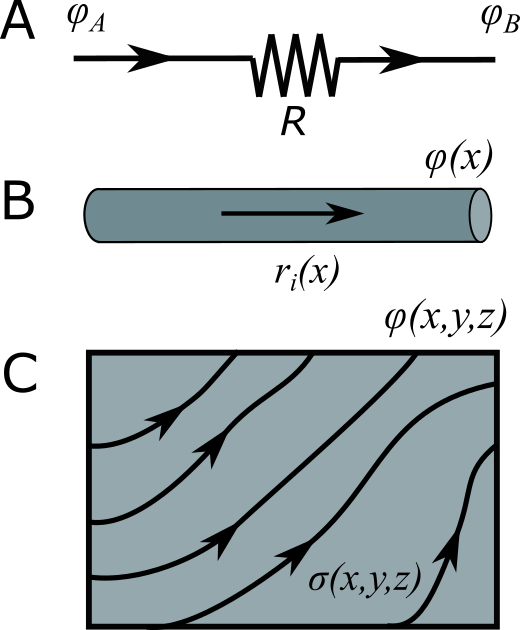
\includegraphics[width=0.6\textwidth]{Figures/Basics/Currents.png}
\end{center}
\caption{{\bf Ohms law for currents and current densities.} {\bf (A)} Current through wire and resistor with resistance $R$ (\si{\ohm}): $I = (\phi_B-\phi_A)/R$. {\bf (B)} Current in wire with specific axial resistance per unit length $r_a$ (\si{\ohm\per\metre}).  $I=- (1/r_a) d\phi/dx$. {\bf (C)} Current density (\si{\ampere\per\square\metre}) in a volume conductor with conductivity $\sigma$ (\si{\siemens\metre}): ${\bf i} = \sigma {\bf E} = - \sigma {\bf \nabla} \phi$.}
\label{fig:Basics:Currents}
\end{figure}

In reality, the resistance of the wire is not strictly zero, but for most standard electrical circuits it is an excellent approximation. However, in some applications, for example if the wire is very long and thin, or if it is made of a less conductive material, it may be necessary to treat it as a continuous resistor. If we define the specific axial resistance per unit length $r_{a}$ (units \si{\ohm\per\metre}), Ohm's law becomes:

\begin{equation}
I = - \frac{1}{r_a}\frac{d\phi}{dx},
\label{eq:Basics:Ohm_r}
\end{equation}
where $r_a=r_a(x)$ may in principle vary along the wire (\fref{fig:Basics:Currents}B). With \fref{eq:Basics:Ohm_r}, the potential $\phi(x)$ will vary gradually along the wire. If $r_a$ is constant along the wire, and the wire has length $L$, it is related to the resistance of the total wire through $r_a=R/L$. As we shall see in \fref{sec:Neuron:morphology}, conductive currents running axially through neural dendrites and axons are typically modeled in this manner. 

The examples above were both one-dimensional in the sense that the current was restricted to run exclusively in the direction defined by the wire. In a three dimensional volume, such as for example brain tissue, currents may run in all spatial directions (\fref{fig:Basics:Currents}C). It is then convenient to describe them in terms of a current density, ${\bf i}$ (units \si{\ampere\per\square\metre}), a vector that defines the current per unit cross section area and its spatial direction. The current density\index{Current density} can be defined in all points in 3D space, and is not dependent on any particular and predefined cross-section area. The conductive properties of a material can be specified either through its resistivity $r$ (units \si{\ohm\metre}), or its inverse, the conductivity $\sigma$ (units \si{\siemens\per\metre}), both being material properties. We shall here use the latter convention, and with that, Ohm's law takes the form:
\begin{equation}
{\bf i} = - \sigma {\bf \nabla} \phi
\label{eq:Basics:Ohm_3D_phi}
\end{equation}
%
On a more general form, Ohm's law states that:
\begin{equation}
{\bf i} = \sigma {\bf E}.
\label{eq:Basics:Ohm_general}
\end{equation}
In comparison, \fref{eq:Basics:Ohm_R}-\fref{eq:Basics:Ohm_3D_phi} hold only in the cases when the electric field ${\bf E}$ can be expressed as a gradient of the potential (cf. \fref{eq:Basics:EV}), which we shall assume throughout this book. A discussion of this assumption is given in \fref{sec:VC:quasistatic}.


\subsubsection{\blue{A note on Ohms law}}
\label{sec:Basics:Note}
It is important to remember that Ohm's law (\fref{eq:Basics:Ohm_general}) represents the average movement of charge on larger spatial scale, and does not apply for movement of individual charges on the nanometre scale. If we compare it with the fundament for electric interactions it is easy to get confused, so let us dive into that confusion and try to clear it up. According to \fref{eq:Basics:E}, an electric field acts on a reference charge $q$ by a constant force, and should according to Newton's law (${\bf F} = m{\bf a}$) give it a constant acceleration in the field-direction. Conversely, \fref{eq:Basics:Ohm_general} states that ${\bf E}$ gives rise, not to a constant acceleration of charges, but rather a constant current, i.e., a constant average \textit{velocity} of charges.

The reason for the discrepancy between the single charge (constant acceleration) and many-charge (constant velocity) scales is that the constant acceleration (eq. \ref{eq:Basics:E}) of our single protagonist charge $q$ will go on for only a tiny time period (the charge relaxation-time) \index{Charge-relaxation} before it will bump into some other particle and be scattered out in some random direction. After the scattering event, the acceleration will start "from scratch", and go on until the next collision takes place, and so forth. Whereas the scattering events will tend to make the motion of $q$ a random walk (which should give it a zero average velocity in any preferred direction), the small periods of acceleration between collisions will at average give $q$ a net drift velocity in the field direction. As the same will happen for all other charges present, there will be a net drift of charge in the field direction. The current density given by \fref{eq:Basics:Ohm_general} is therefore often referred to as the \textit{drift current density}\index{Drift current}. Admittedly, the explanation that we proposed here was somewhat hand-waving, and the fact that we get the linear (constant velocity) relationship in \fref{eq:Basics:Ohm_general} is constitutive, meaning that it is observed experimentally rather than derived from first physical principles. It is found to be a good approximation for many mediums under many conditions, and an excellent approximation for brain tissue \cite**{Nunez2006,Pettersen2012}.


\subsection{\blue{Capacitive currents}}
\label{sec:Basics:CapacitiveCurrent}
\index{Capacitive current}
A common element in electrical circuits is the capacitor. Capacitors are devices that can store electric charge. The simplest form of a capacitor, a parallel plate capacitor, consists of two electrical metallic plates or surfaces separated by an insulating (dielectric) medium\index{Dielectric medium}. By definition, a dielectric medium is one where charges are bound to stay in confined regions of space. An electric field will only slightly shift their average equilibrium positions, causing a polarization of the material. 

A parallel plate capacitor can separate a charge $q$ on one plate from a charge $-q$ on the other plate, to obtain a voltage difference:
\begin{equation}
\phi = \frac{q}{C},
\label{eq:Basics:Vcap}
\end{equation}
where $C$ (units Farad (\si{\farad} = \si{\coulomb\per\volt})) is the capacitance.

To understand how a capacitor works, consider the illustration in \fref{fig:Basics:Capacitor}, where a conductive current $I_\text{in}$ enters the capacitor from the left, and a conductive current $I_\text{out}$ leaves to the right. Kirchhoff's current law states the current flowing into any node in a circuit must equal the current flowing out from that node, which means that we must define
a \textit{capacitive current} $I_\text{cap}$ over the capacitor, so that we get continuity: $I_\text{in} = I_\text{cap} = I_\text{out}$.

\begin{figure}[!ht]
\begin{center}
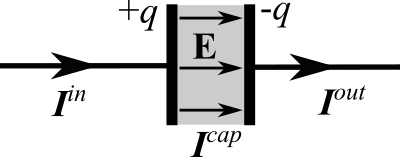
\includegraphics[width=0.6\textwidth]{Figures/Basics/Capacitor.png}
\end{center}
\caption{{\bf Capacitor}.  In the simplest form, a capacitor consists of two electrical metallic plates or surfaces separated by an insulating (dielectric) medium. Charges $q$ and $-q$ on the metal plate generate an electric field $E$ in the dielectric medium, or a potential difference, $\phi = Ed$ where $d$ is the distance between the metal plates. We skipped the vector notation on $E$ since the field direction is implicit.
}
\label{fig:Basics:Capacitor}
\end{figure}

Whereas the conductive currents $I_\text{in}$ and $I_\text{out}$ are mediated by charges moving freely through cables, no charges actually move across the capacitor itself. Instead, $I_\text{in}$ leads to an accumulation of charge $dq/dt$ on the left metal plate of the capacitor. This, in turn, evokes an electric field across its dielectric core, which drives positive charges away from the rightmost metal plate, charging it negatively $-dq/dt$. The temporal rate of change of the electric field across the dielectric medium can be described in terms of a capacitive current defined by:

\begin{equation}
I_\text{cap} = \frac{dq}{dt} = C\frac{d\phi}{dt},
\label{eq:Basics:Icap}
\end{equation}
Although $I_\text{cap}$ differs from conductive currents in the sense that it does not involve free transfer of charge through a medium, it has the same units (A).

The capacitive current was introduced here because neural membranes have capacitive properties, which causes the neural membrane potential to change when currents pass through the membrane. It is customary to express the capacitive membrane current in terms of a current density:

\begin{equation}
i_\text{cap} = c_m\frac{d\phi_m}{dt},
\label{eq:Basics:Icap_mem}
\end{equation}
where $c_\text{m}$ (units \si{\farad\per\square\metre}) is the capacitance per unit membrane area. In this case, the current density is one-dimensional and in the direction normal to the membrane.


\subsection{\blue{Diffusive currents}}
\label{sec:Basics:DiffusiveCurrent}
\index{Diffusion} \index{Diffusive current}
The charge carriers in the brain are ions floating around in the saline solutions that fill up the intra- and extracellular spaces. Ions in salt water will, like electrons in a metal conductor, be accelerated by the presence of an electric field, and will thus carry conductive currents in accordance to Ohm's law (\fref{eq:Basics:Ohm_general}).

In addition to movement propelled by the electric field, ions in water may also move due to diffusion. If the concentration ($c_k$) of an ion species $k$ varies with position, there will be a net transfer of ions towards regions with low concentration, and since ions carry electric charge, this movement amounts to an electric current that comes in addition to the conductive current. 

The electrodiffusive \index{Electrodiffusion} nature of ionic motion is described by the Nernst-Planck equation\index{Nernst-Planck equation},
\begin{equation}
{\bf j}_k = - D_k {\bf \nabla} c_{k} - \frac{D_k z_k c_k}{\psi} {\bf \nabla} \phi,
\label{eq:Basics:JNP}
\end{equation}
which determines the flux density, ${\bf j}_k$ (units \si{\mole\per\square\metre\per\second}) of an ion species $k$. The first term on the right hand side of \fref{eq:Basics:JNP} is Fick's law for diffusion, and states that the diffusive flux of ion species $k$ is proportional to the diffusion constant ${D}_k$ (units \si{\square\metre\per\second}) times the concentration gradient ${\bf \nabla} c_{k}$. ${D}_k$ is a property of the medium that the ion diffuses through, and determines how "easy" it is for the ion $k$ to move through the medium. The second term on the right hand side of eq. \ref{eq:Basics:JNP} accounts for ionic drift due to the electric field. The factor $D_k/\psi$ is the electrical mobility of the ions, which is linearly related to their diffusion constant. This linear relationship is called the Einstein relation\index{Einstein relation}. It does not apply generally, but is valid for dilute solutions, such as the saline solutions in the brain \cite**{Grodzinsky2011}. The valency, $z_{k}$, is a unit-less number that denotes the number of unit charges associated with a single ion of species $k$. The factor $\psi=RT/F$ (units \si{\volt}) is defined by the gas constant ($R = 8.314 \, \si{\joule\per\mole\per\kelvin}$), Faraday's constant ($F = 96458.3\, \si{coulomb\per\mole}$), and the temperature ($T$ with units \si{\kelvin}).

Faraday's constant is defined as the charge per mole ($6.02\times10^{23}$) of unit charges. A flux density ${\bf j_k}$ can thus be converted to a current density by multiplying it with $Fz_k$. A salt water solution is composed of several ions, and to obtain the net electric current, we can sum over the contributions from all of them to obtain the total current density:
\begin{equation}
{\bf i} = \sum_k z_k F {\bf j}_k = -\sum_k{F z_k {D_k}{\bf \nabla} c_{k}} - F\sum_{k} \frac{{D_k} z_{k}^2}{\psi}c_{k} {\bf \nabla}{\phi}.
\label{eq:Basics:iNP}
\end{equation}
The last term on the right hand side is the drift current density,
\begin{equation}
{\bf i}_\text{drift} = - F\sum_{k} \frac{{D_k} z_{k}^2}{\psi}c_{k} {\bf \nabla}{\phi} = - \sigma {\bf \nabla}{\phi}.
\label{eq:Basics:idrift}
\end{equation}
As we indicated with the last equality, the drift current density is the same as the Ohmic current that we defined in eq. \ref{eq:Basics:Ohm_3D_phi}, which means that we can identify the conductivity $\sigma$ of a salt water solution as:
\begin{equation}
\sigma = \frac{F}{\psi}\sum_{k} {D}_k z_{k}^2 c_{k},
\label{eq:Basics:sigma_conc}
\end{equation}

The first term on the right hand side of \fref{eq:Basics:iNP} is the diffusive current density,
\begin{equation}
{\bf i}_\text{diff}  = -\sum_k{F z_k {D_k}{\bf \nabla} c_{k}}.
\label{eq:Basics:idiff}
\end{equation}
Hence, in a conductive medium that contains concentration gradients, the total current is not purely Ohmic, but can contain an additional contribution from ionic diffusion. 

In many cases, the total current will be dominated by the drift component, and although it is possible that it sometimes plays a role, it is common to assume that the diffusive component is negligible when modeling extracellular currents in the brain. The diffusive current does, however, play an important role over neuronal membranes.


\subsection{\blue{Other currents}}
\fref{sec:Basics:OtherCurrents}
Generally, currents additional to those defined above may arise due to advection or magnetic induction. An advective current\index{Advective current},
\begin{equation}
{\bf i}_\text{adv} = F \rho {\bf u},
\label{VC:eq:iadv}
\end{equation}
arises in a bulk solution if the solution has a charge density $\rho$ that it drags along with it due to a bulk flow with velocity ${\bf u}$. However, as we argued in \fref{sec:Basics:Debye}, the saline solution in the brain is practically electroneutral ($\rho \simeq 0$), and the advective current therefore becomes negligible. A more thorough argument for this was given in \citeasnoun**{Gratiy2017}.

As we briefly touched upon earlier, charges may also be accelerated by changes a magnetic field ${\bf B}$, which gives rise to so-called inductive current proportional to $\partial {\bf B}/\partial t$. However, in the brain, inductive currents are assumed to be of negligible importance (more about this in \fref{sec:Basics:Maxwell}).




%%%%%%%%%%%%%%%%%%%%%%%%%%%%%%%%%%%%%%%%%%%%%%
\section{\blue{Extracellular potentials in the brain}}
\label{sec:Basics:ECSpot}
The main focus in this book is on modeling and interpreting extracellular potentials in the brain. As we indicated earlier, an expression for the extracellular potentials originating from neural activity can be derived from the principle of current continuity. 
Let us therefore start this endeavor by defining the types of currents that are relevant in different components of brain tissue.

\subsection{\blue{Electric currents in the brain}}
\label{sec:Basics:braincurrents}
Having introduced different kinds of currents in \fref{sec:Basics:Current}, we can now summarize the role that they play within a brain-specific context. It is useful to make a distinction between currents existing in one of three different mediums, running through either:
\begin{itemize}
\item The intracellular saline solution (cytosol)
\item The extracellular saline solution
\item The cellular (neuronal or glial) membrane
\end{itemize}

Among these three, the membrane currents are the odd ones out. A bit cartoonishly, we may think of the cellular membrane as an insulator (dielectric medium) with small holes. Due to its dielectric properties, it can store charges in so-called Debye-layers on its in- and outside, in a way equivalent to how charges are stored on the metal plates in a parallel plate capacitor (cf. \fref{fig:Basics:Capacitor}). This charge-storage process can be described in terms of a capacitive current like that defined in by \fref{eq:Basics:Icap_mem}, which causes the membrane potential to vary with time. The holes represent various kinds of ion channels, which are conductive pores in the membrane that allow ions to pass through them. Ionic currents through ion channels come in addition to the capacitive current. The capacitive and conductive membrane currents are both essentially one-dimensional and perpendicular to the membrane. They depend both on voltage- and ion concentration differences between the inside and outside of the membrane, and are thus electrodiffusive in their nature, cf. \fref{eq:Basics:iNP}, but in one dimension, so that ${\bf \nabla} \rightarrow d/dx$.

The intra- and extracellular currents are generally three-dimensional electrodiffusive volume currents (cf. \fref{eq:Basics:iNP}) through the conductive saline solutions that fill up the intra- and extracellular spaces. However, as concentration gradients within the intracellular and extracellular spaces typically are much smaller than those across membranes, it is common to neglect the diffusive component, and approximate the intra- and extracellular currents as being purely conductive (cf. \fref{eq:Basics:Ohm_3D_phi}). An illustration of the involved currents in a small piece of tissue is given in \fref{fig:Basics:Twostep}A. As indicated there, currents travel in loops, so that the intracellular and extracellular currents are coupled through the transmembrane currents at the cellular boundary. 

For intracellular currents it is common to make the further simplification that they are well approximated as one-dimensional (cf. eq. \ref{eq:Basics:Ohm_r}). This is motivated by the morphological structure of neurons, which to a fair degree of accuracy can be represented as one-dimensional branching cables of varying diameter (\fref{fig:Basics:Twostep}B).

\begin{figure}[!ht]
\begin{center}
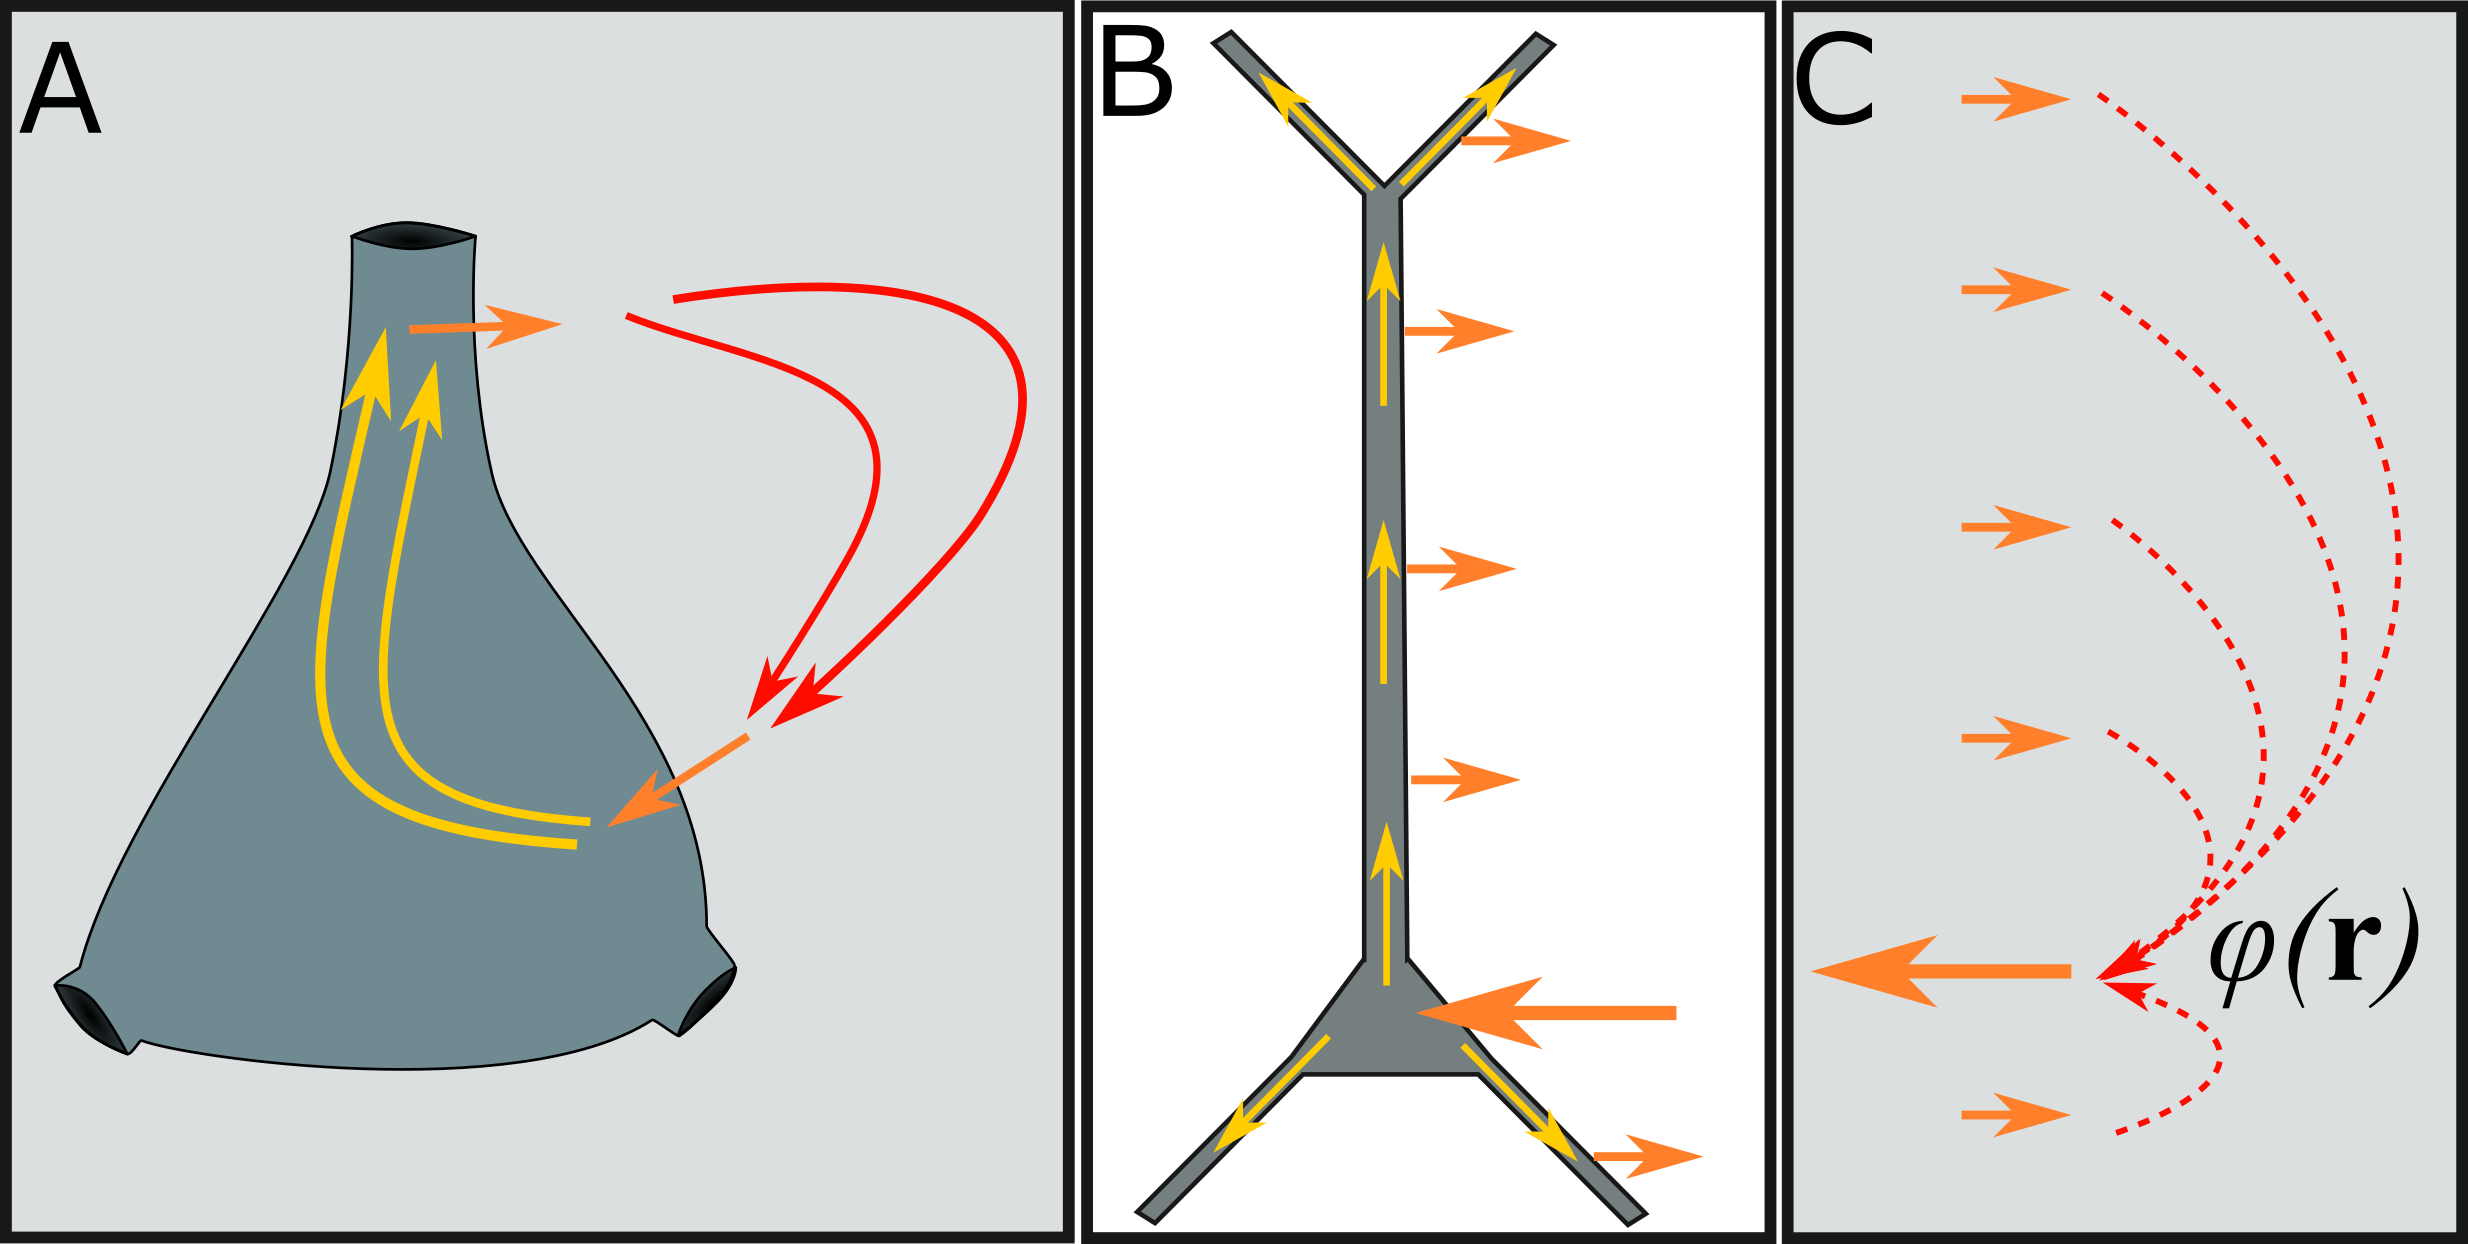
\includegraphics[width=1.0\textwidth]{Figures/Basics/Twostep.png}
\end{center}
\caption{{\bf Currents in brain tissue}. {\bf(A)} Illustration of currents involved in the brain, with intracellular volume currents (yellow), extracellular volume currents (red), and transmembrane currents (orange). Currents travel in closed loops. The entire space will be filled with currents, and only a few paths was included in the illustration. {\bf(B)} A standard modeling strategy is to compute the intracellular and transmembrane currents on a framework independent of the extracellular dynamics. The neuron is approximated as a branching cable, and intracellular currents are one-dimensional along the cable, whereas transmembrane currents are perpendicular to the cable and distributed over the cable. {\bf(C)} The transmembrane currents computed in the framework {\bf(B)} can be used as output sources and sinks to the extracellular space, and can be used to compute the extracellular potential $\phi({\bf r})$. This will be the potential that is "needed" to complete all current loops, a few of which are illustrated with red, dashed arrows.
}
\label{fig:Basics:Twostep}
\end{figure}


\subsection{\blue{Spatial scales}}
\label{sec:Basics:ECSpot}
The recording of an electric potential requires an electrode, and the spatial extension of the electrode determines the spatial resolution of the recording. For example, an electrode placed in the extracellular space of the brain will record the average potential taken over the interface (typically a metal surface or liquid junction) between the electrode and the extracellular fluid, which normally is at least 1~\si{\square\micro\metre}. When we speak of an electric field or potential, we generally mean the average of these quantities taken over a certain volume of interest. 

We started this chapter on the spatial scale of a single atom (\fref{sec:Basics:Charge}). Single charge interactions, taking place on the spatial scale of the Debye-length ($\sim 1 \, \si{\nano\metre}$) and temporal scale of the charge-relaxation time ($\sim 1 \, \si{\nano\second}$), may be important for understanding detailed properties in cellular membranes. However, in this book we are interested in processes on the larger spatial scale where it is meaningful to work with continuous variables such as ion concentrations, charge densities, particle fluxes and electric currents (\fref{sec:Basics:Charge}). 

The Na$^{+}$ concentration in the extracellular space of the brain is $\sim 150 \, \si{\milli\molar}$, which means that a volume of $1 \, \si{\cubic\nano\metre}$ of extracellular space then contains (on average) only $150\times 6.02\times10^{23}\times10^{-27} \approx 0.1$ Na$^{+}$ ions. A concentration is therefore not a very meaningful concept on a spatial scale as small as this. Continuous variables such as ion concentrations, charge densities, particle fluxes and electric currents, therefore imply a spatial resolution $\gg 1 \, \si{\nano\metre}$. When working on this scale, we do not need to be concerned with details of single charge interactions taking place on the nanometre and nanosecond timescale \cite**{Grodzinsky2011}.

When we study processes on the level of brain tissue, we often wish to work on an even coarser spatial scale, using an averaging volume $\gg 1 \, \si{\cubic\micro\metre}$. The diameter of a neural dendrites is typically $\sim 1 \,\si{\micro\metre}$, which means that the averaging volume encloses components of multiple neurites, and includes both intra- and extracellular spaces. The advantage with such a \textit{coarse-grained}\index{Coarse-grained} resolution, is that both cellular and extracellular currents will be defined over the whole tissue-space, rather than within their respective sub-spaces \cite**{Gratiy2017}. At this spatial scale, the intracellular current, for example, does not interpret as belonging to a specific neuron, but rather as the average intracellular current within the whole volume, containing contributions from several different neurons. Likewise, also the transmembrane currents and extracellular currents are volume averages. 


\subsection{\blue{Neurons as current sources}}
\label{sec:Basics:C}
\index{Current source density}
Although potentials fundamentally are due to the distribution of charges on a nanometre scale, the shielding effects that we discussed in \fref{sec:Basics:Debye} allow us to predict a macroscopic (coarse-grained) extracellular potential from the constraint that there should be no charge accumulation anywhere in the extracellular space, or equivalently, that there should be no net electric current entering or leaving any finite volume of tissue.

On the coarse-grained tissue scale ($\gg 1 \,\si{\cubic\micro\metre}$), a common starting point for computing extracellular potential is the requirement that all currents entering or leaving through neuronal membranes must somehow be conserved and distributed in the extracellular space. This can be expressed mathematically through the continuity equation \cite**{nicholson1975}:
\begin{equation}
{\bf \nabla} \cdot {\bf i}_\text{t} = -C,
\label{eq:Basics:continuity1}
\end{equation}
where the source term, $C$ (with units \si{\ampere\per\cubic\metre}), is called the current source density (CSD). The CSD represents the transmembrane output currents from neurons per tissue volume and includes both the capacitive and conductive membrane currents. We have let ${\bf i}_\text{t}$ denote the density of current running extracellularly through brain tissue. It does not include intracellular or transmembrane neural currents.

In a volume of space where there is no transmembrane currents ($C = 0$), \fref{eq:Basics:continuity1} reduces to ${\bf \nabla} \cdot {\bf i}_\text{t} = 0$, which means that there will be no net tissue current entering or leaving such a volume. Importantly, this does not mean that the tissue current must be zero. Currents can still run \textit{through} the volume, as long as the amount of current entering equals the amount leaving it. In a volume that \textit{does} receive transmembrane currents, \fref{eq:Basics:continuity1} tells us that the current outputted from the neuron into that volume ($C$) must be carried away from that volume in terms of an extracellular tissue current. As we shall show in \Fref{chap:VC}, this conservation law shall be the foundation for modeling extracellular potentials arising from neural activity.

For most parts of this book, we shall approximate brain tissue as a \textit{linear} Ohmic conductor, an approximation that we will discuss in further detail below. This means that the tissue current densities are given by Ohm's law for volume conductors (\fref{eq:Basics:Ohm_3D_phi}). When this is inserted into \fref{eq:Basics:continuity1}, we obtain a relationship between the neuronal current sources and the extracellular potential:
\begin{equation}
{\bf \nabla} \cdot \left(\sigma_\text{t} {\bf \nabla} {\phi} \right) = -C,
\label{eq:Basics:continuity2}
\end{equation}
where we have used the index $t$ to denote that $\sigma_\text{t}$ is the \textit{tissue} conductivity. If $\sigma_\text{t}$ does not vary across space, this simplifies to the often used form:
\begin{equation}
\sigma_\text{t} \nabla^2{\phi} = -C.
\label{eq:Basics:continuity3}
\end{equation}


\subsubsection{\blue{Derivation of the CSD equation}}
\label{sec:Basics:C2}
\index{Current source density}
Although  \fref{eq:Basics:continuity1} may seem intuitively reasonable, we introduced it above more or less as a postulate. A thorough derivation of this equation was given by \citeasnoun**{Gratiy2017}, and for the interested reader, we will here go through the main steps of this derivation. 

In general, current conservation implies that: 
\begin{equation}
{\bf \nabla} \cdot {\bf i}_\text{tot} = 0, 
\label{eq:Basics:Sergey1}
\end{equation}
where we can think of ${\bf i}_\text{tot}$ as the total current density defined on the relatively fine spatial scale where it is meaningful to distinguish between it being either cellular or extracellular. Let us further define $\left<\cdot {\bf i}_\text{tot}\right>$ as being this total current when averaged over some coarse-grained volume that spans over both intra- and extracellular spaces. 
As current conservation also applies at this scale, we have that: 
\begin{equation}
{\bf \nabla} \cdot \langle{\bf i}_\text{tot}\rangle = 0.
\label{eq:Basics:Sergey2}
\end{equation}
Since we may perform the averaging separately over the cellular (c) and extracellular (e) domains, we have that $\langle{\bf i}_\text{tot}\rangle = \langle{\bf i}_\text{tot}\rangle_\text{c} = \langle{\bf i}_\text{tot}\rangle_\text{e}$. With this, we can may write \fref{eq:Basics:Sergey2} as:
\begin{equation}
{\bf \nabla} \cdot \langle{\bf i}_\text{tot}\rangle_\text{c}  + {\bf \nabla}\cdot \langle{\bf i}_\text{tot}\rangle_\text{e} = 0
\label{eq:Basics:Sergey3}
\end{equation}
In Appendix A of \citeasnoun**{Gratiy2017}) it was shown that the that the divergence of the coarse-grained current density over the cellular domain can be expressed as a sum of transmembrane currents (i.e., as the CSD term ($C$) that we introduced in \fref{eq:Basics:continuity1}. Further, if we rename the average current running extracellularly through tissue $\langle{\bf i}_\text{tot}\rangle_\text{e}$ to ${\bf i}_\text{t}$, we see that \fref{eq:Basics:Sergey3} becomes identical to  \fref{eq:Basics:continuity1}. 

The derivation of \fref{eq:Basics:continuity1} thus reveals that it only has a meaningful interpretation when considering tissue in a coarse-grained scale, i.e., a spatial scale large enough to contain both intra- and extracellular domains. Importantly, ${\bf i}_\text{t}$ thus interprets as the average current running extracellularly through tissue, defined as extracellular current per unit \textit{tissue} cross section area and not per \textit{extracellular} cross section area (although it only runs through the extracellular parts of this cross section area). Similarly, $\sigma_\text{t}$ in \fref{eq:Basics:continuity2} interprets as average conductivity experienced by the current ${\bf i}_\text{t}$. As this current will face cellular obstacles, and is restricted to run only through the extracellular parts of the tissue, $\sigma_\text{t}$ is generally lower than the conductivity of the extracellular saline solution (see \fref{chap:Sigma} for further discussion). 


\subsection{\blue{Two-step approach for modeling extracellular potentials}}
\label{sec:Basics:twostep}
To compute extracellular potentials using \fref{eq:Basics:continuity2}, we need to know the neuronal output current $C$. Generally, the transmembrane currents in neurons depend on the membrane potential $\phi_\text{m}$, defined as the difference between the intracellular ($\phi_\text{i}$) and the extracellular ($\phi_\text{e}$) potentials immediately inside and outside the membrane. Hence, in principle, transmembrane currents depend on extracellular potentials, and the extracellular potential in turn depends on the transmembrane currents of all nearby neurons. As it is very challenging to simulate all these variables simultaneously in a self-consistent manner, standard modeling approaches are based on the simplifying assumption that the neurodynamics is independent of the extracellular potential. Since the transmembrane potential ($\sim -70 \, \si{\milli\volt}$ tends to be much bigger than extracellular potentials ($\sim 1 \,\si{\milli\volt}$), this is mostly a reasonable approximation (but see \fref{sec:Neuron:HHCassumptions} for a further discussion). One may then take a two-step approach to model the cellular and extracellular dynamics:

\begin{itemize}
\item {\bf Step 1:} Compute the cellular dynamics (intracellular currents, membrane currents, and membrane potential) using a separate framework based on the assumption that this is independent on what goes on in the extracellular space (Fig. \ref{fig:Basics:Twostep}B).

\item {\bf Step 2:} Use the transmembrane currents computed in Step 1 as "external" input currents (sinks and sources) $C$ to the extracellular space (Fig. \ref{fig:Basics:Twostep}C). Based on \fref{eq:Basics:continuity2}, with $C$ as obtained in Step 1, an analytical formula can be derived for how the set of transmembrane currents give rise to an extracellular potential $\phi({\bf r})$.
\end{itemize}

Throughout this book, we shall use this two-step approach to compute extracellular potentials, but we will briefly introduce the theory behind alternative and more physically detailed frameworks. The standard framework for completing Step 1 is presented in \Fref{chap:Neuron}, and we will refer to it as the multicompartment (MC) framework, as it is based on multicompartment models of neurons. The standard framework for completing Step 2 is the volume conductor (VC) theory presented in  \Fref{chap:VC}.



\section{\blue{Maxwell's equations}}
\label{sec:Basics:Maxwell} \index{Maxwell's equations}
The physics of electromagnetism is summarized by Maxwell's equations, so we end this chapter by going briefly through these. We will also discuss some of the approximations of Maxwell's equations that we use when applying them to studies of brain tissue.

Maxwell's equations come in two versions, referred to as the microscopic and macroscopic versions. The microscopic version is the most fundamental, but using it requires knowledge of the positions of all individual charges. Since that is unfeasible when any medium at a macroscopic level, we therefore only list up the macroscopic set of equations:

\begin{eqnarray}
{\bf \nabla}\cdot {\bf D} & = & \rho, \label{eq:Basics:Max11} \\
{\bf \nabla} \cdot {\bf B} & = & 0,   \label{eq:Basics:Max22} \\
{\bf \nabla} \times {\bf E} & = & - \frac{\partial {\bf B}}{\partial t},  \label{eq:Basics:Max33} \\
{\bf \nabla} \times {\bf H} & = & {\bf i}_\text{free} + \frac{\partial {\bf D}}{\partial t}.  \label{eq:Basics:Max44}
\end{eqnarray}
Here $\rho$ and ${\bf i}_\text{free}$ are the free (unbound) charge and current densities, as the influence of bound charge and current is incorporated in the the auxillary displacement and magnetizing fields, ${\bf D}$ and ${\bf H}$. For linear mediums, ${\bf D}$ and ${\bf H}$ can be expressed in terms of the fundamental magnetic (${\bf B}$, with units tesla (\si{\tesla})) and electric (${\bf E}$) fields through the constitutive relations\index{Constitutive relations} ${\bf B} = \mu{\bf H}$ and ${\bf D} = \epsilon {\bf E}$, where $\mu$ (units henries per metre (\si{\henry\per\metre})) is the magnetic permeability of the medium and $\epsilon$ (units \si{\farad\per\metre}) the electric permittivity of the medium. By \textit{constitutive relations}, we simply mean relations that are observed experimentally to be good approximations for a specific material. They are known to be excellent approximations for brain tissue \cite**{Nunez2006}. Maxwell's equations then take the form:

\begin{eqnarray}
{\bf \nabla}\cdot {\bf E} & = & \frac{\rho}{\epsilon}, \label{eq:Basics:Max1} \\
{\bf \nabla} \cdot {\bf B} & = & 0,  \label{eq:Basics:Max2} \\
{\bf \nabla} \times {\bf E} & = & - \frac{\partial {\bf B}}{\partial t}, \label{eq:Basics:Max3} \\
{\bf \nabla} \times {\bf B} & = & \mu {\bf i}_\text{free} + \mu\epsilon\frac{\partial {\bf E}}{\partial t}.  \label{eq:Basics:Max4}
\end{eqnarray}

\Fref{eq:Basics:Max1} is Gauss's law (for electricity). The free charge density, $\rho$, can generally be non-zero, although we argued earlier that brain tissue for practical purposes can be assumed to be electroneutral at the coarse-grained scale.

\Fref{eq:Basics:Max2} is Gauss's law for magnetism, and is the magnetic equivalent to eq. \ref{eq:Basics:Max1}. Whereas eq. \ref{eq:Basics:Max1} allows a spatial gradient of the electric field due to a local charge density $\rho$, eq. \ref{eq:Basics:Max1} disallows the corresponding gradient in the magnetic induction field. That is because magnetic monopoles do not exist\gex{, at least outside France.}

\Fref{eq:Basics:Max3} is the Maxwell-Faraday equation for electromagnetic induction. The cross product ${\bf \nabla} \times {\bf E}$ represents a certain kind of change in the electric field called the \textit{curl}. The equation tells us that such a change will be induced if there is a temporal variation in the magnetic field.

\Fref{eq:Basics:Max4} is Ampere's circuital law, and is the magnetic equivalent to \fref{eq:Basics:Max3}. According to \fref{eq:Basics:Max4}, a magnetic field will be induced either by an electric current of free charges going through the medium (first term on the right), or by a temporal change in the displacement field (second term on the right). The last term is often called the displacement current. The Ohmic current that we introduced earlier (\fref{eq:Basics:Ohm_general}) is an example of a current of free charges, while the capacitive current that we introduced earlier (\fref{eq:Basics:Icap_mem}) is an example of a displacement current, where the capacitance can be expressed as a function of $\epsilon$.

It is interesting to note that the principle of current and charge conservation follows directly from Maxwell's macroscopic equations.To see this, we may start with taking the divergence (${\bf \nabla} \cdot$) of both sides of eq. \ref{eq:Basics:Max4}. Since the divergence of a cross product is always zero, \fref{eq:Basics:Max4} then reduces to:
\begin{equation}
{\bf \nabla} \cdot \left( {\bf i}_\text{free} +  \epsilon \frac{\partial {\bf E}}{\partial t} \right) = 0.
\label{eq:Basics:Max4dot}
\end{equation}
This equation states that the total current (${\bf i}_\text{tot} = {\bf i}_\text{free} +  \epsilon \frac{\partial {\bf E}}{\partial t}$) into any volume of space must be zero. To see the charge conservation explicitly, we can insert \fref{eq:Basics:Max1} for ${\bf E}$ to obtain:
\begin{equation}
- {\bf \nabla} \cdot {\bf i}_\text{free} =  \frac{\partial \rho}{\partial t}.
\label{eq:Basics:currentconservation}
\end{equation}
Hence, if the left hand side in nonzero, there is a net influx of free charges into a volume, and if that is the case, there must be an accumulation of charge there, as described by the right hand side of the equation. This equation thus reveals the equivalence between the displacement current (last term on the right hand side of \fref{eq:Basics:Max4dot}) and a local accumulation of free charge (left hand side of \fref{eq:Basics:currentconservation}).


\subsection{\blue{Quasi-static approximations of Maxwell's equation}}
\label{sec:Basics:Quasistatic} \index{Quasi-static approximation}
Together, Maxwell's equations give a unified theory for electricity and magnetism, and laid the theoretical fundament for understanding electromagnetic radiation such as light. We can "see the light" by looking at \fref{eq:Basics:Max3} and \fref{eq:Basics:Max4}. \Fref{eq:Basics:Max3} shows that a temporal change in the magnetic field induces an electric field perpendicular to the change (perpendicular, because that is what the curl-operation ${\bf \nabla} \times$ does), while \fref{eq:Basics:Max4} shows that a temporal change in the electric field (last term on the right hand side) induces magnetic field perpendicular to the change. Electromagnetic radiation is due to such an interplay where electric and magnetic fields act on each other through a periodic series of inductions and cancellations that propagate as a wave through a medium. 

The generation of such electromagnetic waves are, however, is not a characteristic feature of brain activity. Brain activity at the scale of tissue is therefore often studied using the quasistatic-approximations of Maxwell's equations \cite**{Hamalainen1993}. This means that in the calculation of ${\bf E}$ and ${\bf B}$, the source terms associated with temporal changes in the fields $\partial{\bf B}/\partial t$ and $\partial{\bf E}/\partial t$ are assumed to give a negligible contribution. When making these approximations, the electric and magnetic fields decouple. It is worth mentioning that the \textit{quasi-electrostatic} assumption that $\partial{\bf B}/\partial t \approx 0$ in \fref{eq:Basics:Max3} does not by necessity imply that the \textit{quasi-magnetostatic} assumption that $\partial{\bf E}/\partial t \approx 0$ in \fref{eq:Basics:Max4} must hold, or vice versa. Also, the electric and magnetic fields can be effectively decoupled if only one of them is true. 

The CSD equation (\fref{eq:Basics:continuity2}) that we will use to describe electric fields in the brain rests heavily on the quasi-electrostatic approximation Maxwell's equations, which means that \fref{eq:Basics:Max3} simplifies to:
\begin{equation}
{\bf \nabla} \times {\bf E} \approx 0.
\label{eq:Basics:quasiel}
\end{equation}
A zero curl of the electric field is a prerequisite for expressing ${\bf E}$ as a gradient of a potential, like we did in \fref{eq:Basics:EV}. This approximation has been justified in many works, and is warranted because fields of physiological origin are normally of frequencies below a few thousand \si{\hertz}, and then have a negligible effect on electric fields \cite**{Plonsey1967,Hamalainen1993,Gratiy2017}. 
 
In addition, the CSD equation rests on the approximation that the magnetic fields (wether they vary with time or not) are too small to significantly affect the movement of electric charges. As we briefly mentioned early in this chapter, charges can be accelerated both by electric and magnetic forces, collectively referred to as the Lorenz force:
\begin{equation}
{\bf F} = q({\bf E}) + {\bf u}\times{\bf B},
\label{eq:Basics:Lorenz}
\end{equation}
which adds magnetic component to the electric force that we defined previously in \fref{eq:Basics:E}. Here, {\bf u} (units \si{\metre\per\second}) is the velocity of the charged particle, and the magnetic force is given by the cross product of the vectors ${\bf u}$ and ${\bf B}$, which means that it will act in the direction perpendicular to both of them. At the coarse-grained scale at which the CSD equation (\fref{eq:Basics:continuity2}) applies, the relevant velocity is that of the bulk flow of ions. The maximal blood flow velocity through arteries has been estimated to be $\sim 1 \,\si{\metre\per\second}$ \cite**{bishop1986}, which we can take as an upper limit for the bulk flow velocity. If we combine this with typical fields $B = 10^{-13} \, \si{\tesla}$ \cite**{Hamalainen1993}, and $E = 1 \,\si{\volt\per\metre}$ \cite**{Cordingley1978}, arising from neural activity, we can estimate the ratio between the magnetic and electric force to be $uB/E \sim 10^{-13}$ \cite**{Gratiy2017}. Hence, as we have assumed throughout this chapter, magnetic effects on the movement of charges in brain tissue are negligible. The reason why this is important, is that ${\bf i}_{free}$ in \fref{eq:Basics:Max4dot} then becomes independent of ${\bf B}$, which we implicitly assumed when we used Ohm's law for volume conductors (\fref{eq:Basics:Ohm_3D_phi}) to derive the CSD equation (\fref{eq:Basics:continuity2}). Together, the assumptions that ${\bf \nabla} \times {\bf E} \approx 0$ and $uB \ll E$ are sufficient for electric and magnetic fields to decouple. 

For large scale brain activity, also the quasi-magnetostatic approximation, i.e., that $\partial{\bf E}/\partial t \approx 0$ in \fref{eq:Basics:Max4}, has been shown to be a fairly good approximation \cite**{Plonsey1967,Hamalainen1993}. However, this approximation does not apply to finer spatial scales, as it is the displacement term that gives rise to the capacitive charging of neural membranes \cite**{Gratiy2017}. Also, the quasi-magnetostatic approximation is not a requirement for using the CSD equation on the form (\fref{eq:Basics:continuity2}), as possible capacitive components of the tissue current can be accounted through using a complex tissue conductivity $\sigma_t$ (see \fref{chap:Sigma}).


